\documentclass[]{article}
\usepackage{graphicx}
\graphicspath{ {./images/} }
\usepackage{caption}
\usepackage{subcaption}
\usepackage{amsthm}
\usepackage{amsfonts}
\usepackage{amsmath}
\usepackage{amssymb}
\usepackage{mathrsfs }
\usepackage[ruled,linesnumbered]{algorithm2e}
\newtheorem{mydef}{Definition}[section]
\newtheorem{myproposition}{Proposition}[section]
\newcommand{\mathleft}{\@fleqntrue\@mathmargin0pt}

\title{Master Thesis -- Prove Problem}
\author{Kefang Ding} 
\date{\today}
\begin{document}
\maketitle
\hrulefill
\hrulefill 
\section{Introduction}
This article is used to explain the difficulty I confront about proving the soundness of generated model.
In the first phrase of algorithm, the existing model, positive event log and negative event log are used to generate a new directly-follows graph. Based on Inductiver Miner, this graph is transformed into a sound petri net without long-term dependency. 

In the next phase, our algorithm focuses on detecting and adding long-term dependency in Petri net. We define, if the supported connection on the set pair of xor branches is over a threshold, pair has significant correlation.Therefore, this pair has long-term dependency.

During the implementation, it comes clear that supported connection only on the positive and negative event log is not enough, since the existing model can keep some directly-follows relations about xor branches which do not show in the positive event log or shows only in negative event log. Consequently, when we detect this long-term dependency on those xor branches, there is no evidence of long-term dependency on those xor branches. It results in an unsound model as shown in Fig , since those xor branches can't get fired to consume the tokens generated from the choices before.
%% insert one unsound model here and point out the situations. 
\begin{figure}[!h]
	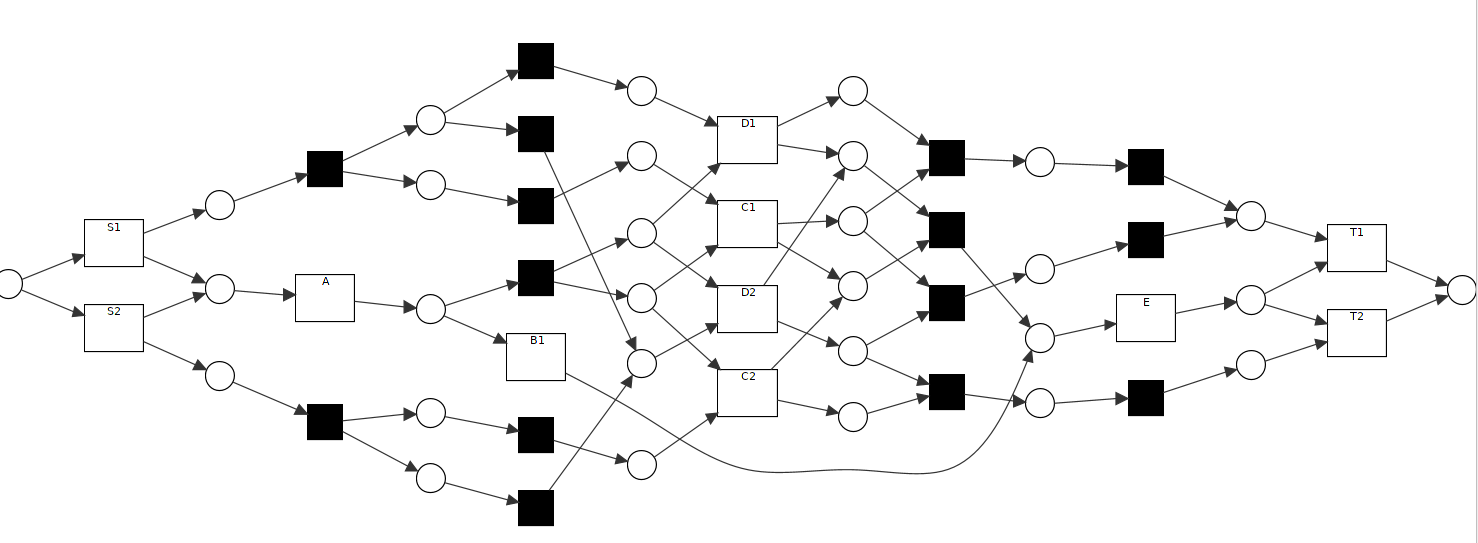
\includegraphics[width=\textwidth]{PN_tc_and_03_01.png}
	\caption{Unsound Repaired Model at Transition B1.}
	\label{fig:unsound_example}
\end{figure}
\section{Problem Description}
To make the generated Petri net sound, we propose a method to incorporate the existing model on the long-term dependency detection. The definition \ref{def: supported-connection} is rephrased into weight. 
\begin{mydef}[Rephrased Correlation of xor branch] The correlation for two branches is expressed into
	\[Wlt(XORB_X,XORB_Y)= Wlt{ext}(XORB_X, XORB_Y) + Wlt{pos}(XORB_X, XORB_Y)\] \[ -Wlt{neg}(XORB_X, XORB_Y)\], where 
	$W_lt{ext}(XORB_X, XORB_Y)= \frac{1}{|XORB_Y*|}$, $|XORB_{Y*}|$ means the number of possible  directly-follows xor branche set $XORB_{Y*}=\{XORB_{Y1}, XORB_{Y2},...XORB_{Yn} \}$ after $XORB_X$. \\ \\
	$Wlt{pos}(XORB_X, XORB_Y)= \frac{F_{pos}(XORB_X, XORB_Y)}{F_{pos}(XORB_X, *)}$, \\
	$Wlt{neg}(XORB_X, XORB_Y)= \frac{F_{neg}(XORB_X, XORB_Y)}{F_{neg}(XORB_X, *)}$, \\	
\end{mydef}
The $F_{pos}(XORB_X, XORB_Y)$ and $F_{neg}(XORB_X, XORB_Y)$ are the frequency of the coexistence of $XORB_X$ and $XORB_Y$, respectively in positive and negative event log.

With this rephrased definition, to make the model sound, we need to prove, if there is a xor branch $XORB_Y$ in the generated process tree, there must exist one long-term dependency related to it, $\exists XORB_X, Wlt(XORB_X,XORB_Y) > lt-threshold$. We formalize this problem. Else, the model can't be sound!!
\begin{myproposition}
	Given a process tree, a pair of xor branch set, $(B_A,B_B)$ with $B_A={XORB_{X1}, XORB_{X2},...XORB_{Xm}}, B_B={XORB_{Y1}, XORB_{Y2},...XORB_{Yn}}$, the obligatory part between $B_A$ and $B_B$ is marked M, it is to prove:: \\
	$\forall XORB_Y \in B_B$, if $W(M, XORB_Yj) > threshold$, \\ then there exists one $XORB_Xi \in B_A$ with 
	\[Wlt(XORB_Xi, XORB_Yj)> lt_threshold\]. 
\end{myproposition}
Given a simplified scenes, it is listed in Fig \ref{fig:simplified-graph-model}. M is an obligatory path from the set $\{X1,X2,..Xm\}$ to $\{Y1,Y2,..Yn\}$. If there exists directly-follows relation of M and Y1, then there must exist one long-term dependency of Xi and Y1. 

\begin{figure}[!h]
	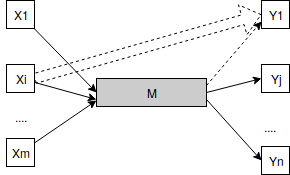
\includegraphics[width=\textwidth]{RelationOfThreshold-LTThreshold.png}
	\caption{Simplified Graph MOdel}
	\label{fig:simplified-graph-model}
\end{figure}

The definition of $W(M, XORB_{Yj})$ is reviewed below.
\begin{mydef}[Assign new weights to graph $G_{new}$]
	there are three weights from $G_{pos}$, $G_{neg}$ and $G_{ext}$, the new weight is 
	\begin{itemize}
		\item For one directly-follows relation, \[ W(E_{G_{new}}(A,B)) = Weight(E_{G_{pos}}(A,B)) + Weight(E_{G_{ext}}(A,B)) - Weight(E_{G_{neg}}(A,B))\]
		\item Given a directly-follows graph G(L), the weight of each directly-follows relation is defined as \[ Weight(E(A,B)) = \frac{Cardinality(E(A,B))}{Cardinality(E(A,*))}  \] 
	\end{itemize}
\end{mydef}

When prove by contradiction, we assume that the opposite proposition is true. If it shows that such an assumption leads to a contradiction, then the original proposition is valid. 
\begin{myproposition}
	for one xor branch $XORB_Y$, if $W(M, XORB_{Yj}) > threshold$, \\ there exists no one $XORB_{Xi}$ with 
	\[Wlt(XORB_{Xi}, XORB_{Yj})<\text{lt-threshold}\]. 
\end{myproposition}

Or we change to another thinking way to get the relation of threshold and lt-threshold, such that we have the theorem valid. Then we rephrase the question into
\begin{myproposition}[Another way of thinking]
	Given a process tree, a pair of xor branch set, $(B_A,B_B)$ with $B_A=\{XORB_{X1}, XORB_{X2},...XORB_{Xm}\}, B_B=\{XORB_{Y1}, XORB_{Y2},...XORB_{Yn}\}$, the obligatory part between $B_A$ and $B_B$ is marked M. If,\\
	for one xor branch $XORB_{Yj}$, if $W(M, XORB_{Yj}) > threshold$, \\ there exists one $XORB_Xi$ with 
	\[Wlt(XORB_{Xi}, XORB_{Yj})> \text{lt-threshold}\]
	What is the relation of threshold and lt-threshold?? 
\end{myproposition}
If we expand the theorem, we need to prove 
\begin{myproposition}[Relation of threshold and lt-threshold]
	What is the relation of threshold and lt-threshold, to make the following proposition valid. If 
	\begin{equation*}
	 \begin{gathered}
		W(M, XORB_{Yj})  > threshold \\
	W(M, XORB_{Yj}) = Weight(E_{G_{pos}}(M, XORB_{Yj})) \\
	+ Weight(E_{G_{ext}}(M, XORB_{Yj})) 
	- Weight(E_{G_{neg}}(M, XORB_{Yj})) \\
	\frac{1}{|Y*|} + \frac{\sum_{Xi}{Cardinality(M,Yj|Xi)}} {\sum_{Xi}{Cardinality(M,Y*|Xi)}}  
	- \frac{\sum_{Xi}{Cardinality(M,Yj|Xi)\prime}} {\sum_{Xi}{Cardinality(M,Y*|Xi)\prime} > threshold} \\
	\text{Then, exist one Yj with}\\
	Wlt(Xi, Yj)> \text{lt-threshold} \\
	Wlt{ext}(Xi, Yj) + Wlt{pos}(Xi, Yj) -Wlt{neg}(Xi, Yj) > \text{lt-threshold}\\
	\frac{1}{|Y*|} + \frac{Cardinality(M,Yj|Xi)} {Cardinality(M,Y*|Xi)}  
	- \frac{Cardinality(M,Yj|Xi)\prime} {Cardinality(M,Y*|Xi)\prime} > \text{lt-threshold}  \\
	\text{Or \textbf{there is a contradiction when all Yj}}\\
	Wlt(Xi, Yj)< \text{lt-threshold}\\
	\sum_{Xi} Wlt(Xi, Yj) < |X*|\bullet \text{lt-threshold} \\
	\frac{|X*|}{|Y*|} + \sum_{Xi}\frac{Cardinality(M,Yj|Xi)} {Cardinality(M,Y*|Xi)}  
	- \sum_{Xi}\frac{Cardinality(M,Yj|Xi)\prime} {Cardinality(M,Y*|Xi)\prime} < |X*|\bullet \text{lt-threshold}  \\
	 \end{gathered}
	\end{equation*}	
$Cardinality(M,Yj|Xi)$ means the frequency of coexistence of M and Yj given Xi in the trace in positive, while $Cardinality(M,Yj|Xi)\prime$ represents the frequency in negative. $Cardinality(M,Y*|Xi)$ is the sum frequency of set ${Y1,..Yj,..Yn}$, it equals to \[Cardinality(M,Y*|Xi) = \sum_{Yi}Cardinality(M,Yj|Xi)\]
\end{myproposition}
If we set them into zero, there is a lot of existing edges kept into the old method with no evidence in event log to support the connection. 
\section{Think out of box}
The main problem is after detecting long-term dependency on the xor blocks, when long-term dependency is added into Petri net by silent transitions and places, will it keep the model sound? By simple examples, we observe the sound model generated from repair method. Yet, with different values of threshold, the new models are unsound. In the following, the questions are proposed. 
\begin{itemize}
	\item In which situations are the generated model sound, or unsound?
	\item What are the reasons behind it ?
	\item If it's unsound, what can be done to improve this method?
\end{itemize}
To deal with those questions, we explain our method to add long-term dependency at first. Some questions are defined formally in the next section. Next, we try to prove the soundness. 
\subsection{The Method Explanation}
After detecting long-term dependency on xor branches from process tree, silent transitions and extra places are added to express those dependency on Petri net. The basic idea is to add control places after $XORB_X$ and control places before $XORB_Y$, then connect those places by silent transition. Due to the structure of xor branches, situations differ, as listed in the Algorithm \ref{alg: Adding method}.  
\begin{algorithm}[!ht]
	\SetAlgoLined
	$XORB_Y$ is dependent on $XORB_X$\;
	\If{$XORB_X$ is leaf node}{
		One place is added after this leaf node. \;
	}
	\If{$XORB_X$ is Seq}{
		Add a place after  the end node of this branch;\;
		The node points to the new place;\;
	}
	\If{$XORB_X$ is And}{
		Create a place after the end node of every children branch in this And xor branch; \; 
		Combine all the places by a silent transition after those places; \;
		Create a new place directly after silent transition to represent the And xor branch; \;
	}
	
	\If{$XORB_Y$ is leaf node}{
		One place is added before this leaf node. \;
	}\If{$XORB_Y$ is Seq}{
		Add a place before  the end node of this branch;\;
		The new place points to this end node;\;
	}\If{$XORB_Y$ is And}{
		Create a place before the end node of every children branch in this And xor branch; \; 
		Combine all the places by a silent transition before those places; \;
		Create a new place directly before silent transition to represent the And xor branch; \;
	}
	Connect the places which represent the $XORB_X$ and $XORB_Y$ by creating a silent transition.
	\caption{Add long-term dependency between pure xor branch}
	\label{alg: Adding method}
\end{algorithm}
Next, we give some examples to show how this method works. We have Model 1 in Fig \ref{fig:pn_without_lt_exm01}, and long-term dependency of 
%% how to express long-term dependency in symbol?? 
%% use multiple graphs to sort 

\begin{figure}[h!]
	\centering
	\begin{subfigure}[b]{\textwidth}
		\centering
		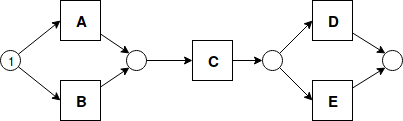
\includegraphics[width=\linewidth]{LT_Seq_01_Original.png}
		\caption{Petri net without long-term dependency}
		\label{fig:pn_without_lt_exm01}
	\end{subfigure}
	\hfill
	\hfill
	\begin{subfigure}[b]{\textwidth}
		\centering
		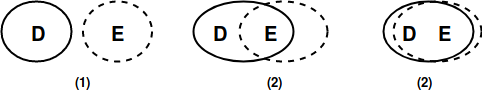
\includegraphics[width=\linewidth]{LT_Seq_01_SetCases.png}
		\caption{long-term situations}
		\label{fig:model_b}
	\end{subfigure}
	\caption{Long-term dependency in Sequence: \small{Solid eclipse represents the set of choices which have long-term dependency with A, while dashed represents the set for B.}}
	\label{fig:lt_seq_examples}
\end{figure}
\begin{mydef}[Control place]
Control Place is the new added place used to express long-term dependency. Its object is one pure xor branch, which means no xor block in its set. It's divided into post control place after source, and pre control place before target. 
According to different types of xor branches, the way to add control places differs as shown in the next Fig. As source, we have post control place after this branch. For leaf node, and Seq branch, post place is connected directly to the last transition; If it is parallel, or loop, place is connected by the silent transition representing the limit of the block. Similarly, pre control places are for the targets.
\end{mydef}
\begin{figure}[!h]
	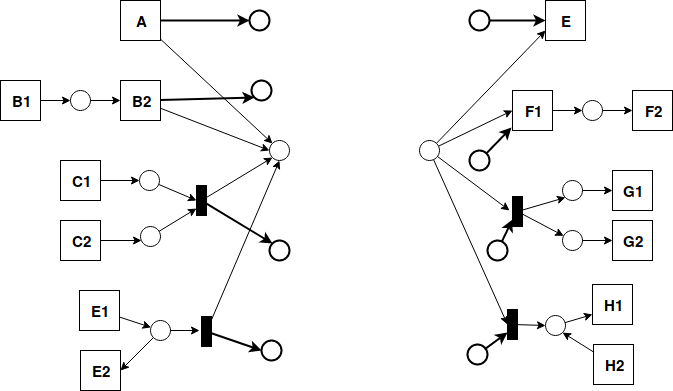
\includegraphics[width=\textwidth]{LT_ControlPlace_01.png}
	\caption{Add long-term dependency in Situation b.1}
	\label{fig:lt_control_place}
\end{figure}
In the situation b.1, given long-term dependency, LT(\{A\})=\{D\}, LT(\{B\})=\{E\}. Since A and B are sources for long-term dependency, control places after A and B are added respectively; D and E are targets in long-term dependency, so the control places are also added before D and E. To express the binary long-term dependency, silent transitions are used to connect the control places from sources and targets. And we get the result in Fig \ref{fig:lt_seq_case_01}.
%% we use the binary situation to express the long-term dependency, so it's binary at first. 
%% So we express the long-term dependency in a form.
\begin{figure}[!h]
	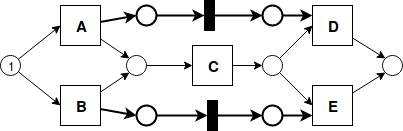
\includegraphics[width=\textwidth]{LT_Seq_01_Case_01.png}
	\caption{Add long-term dependency in Situation b.1}
	\label{fig:lt_seq_case_01}
\end{figure}

In situation b.2, LT(\{A\})=\{D\},LT(\{A\})=\{E\},LT(\{B\})=\{E\}. Post and Pre control places are added only once for the xor branches. Silent transitions are used to express the binary connection. But as we see, A could decide the both D and E, so from post control place, we have two out edges to go to different directions. As for target E, it have source A and B, its pre control place has two incoming edges. 
\begin{figure}[!h]
	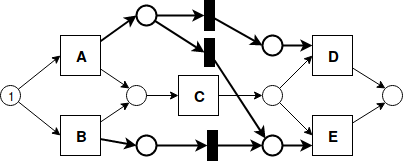
\includegraphics[width=\textwidth]{LT_Seq_01_Case_02.png}
	\caption{Add long-term dependency in Situation b.1}
	\label{fig:lt_seq_case_02}
\end{figure}

In the situation b.3, A and B can decide both execution of D and E, so there is no long-term dependency existing with xor block Xor(A,B) and Xor(D,E). So we keep the model untouched. 

Next we show the strategy to add long-term dependency on xor blocks with either source or target in And. Since two xor blocks Xor(B1,B2), Xor(C1,C2) are in concurrency, so the combination of \{B1,B2\}*\{C1,C2\} will be decided by the choices of Xor(S1,S2) and decides the choices of Xor(T1,T2).
Given long-term dependency, LT(\{S1\})=\{B1,C1\}, LT(\{S1\})=\{B1,C2\} , LT(\{S2\})=\{B1,C2\},  LT(\{S2\})=\{B2,C2\}, LT(\{B1,C1\})=\{T1\}, LT(\{B2,C1\})=\{T1\}, LT(\{B2,C2\})=\{T2\},  LT(\{B2,C2\})=\{T1\}. 
We need to combine the choices at source and target side. 

At source side with multiple transitions, we use silent transition to connect the post places of all transitions in source, the control place is then added after this transition. After this combine transition, we add control place for it. Then Like in Seq situation, we add silent transition to complete the long-term dependency. 

Concurrent xor blocks st target side, control places and combination silent transition are added. After this addition, silent transitions are connected to control places to finish long-term dependency. 
%% draw the pictures to show how do you add silent transition in this situations.
\begin{figure}[!h]
	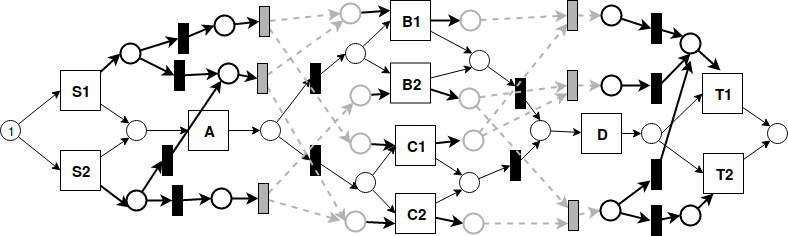
\includegraphics[width=\textwidth]{LT_And_Case_01.png}
	\caption{Add long-term dependency in Situation b.1}
	\label{fig:lt_and_case_01}
\end{figure}
%% what if there is no connection from C2, so not all the place can be reached!!!
The last part describes the long-term dependency on nested xor block. 
If long-term dependency is added to this part, 
\subsection{What to prove?}
\subsection{How to prove}
\subsection{Conclusion}

\end{document}